\documentclass[a4paper]{article}
\usepackage{tabularx}
\usepackage[T1]{fontenc}
\usepackage[utf8]{inputenc}
\usepackage{xcolor}
\usepackage{graphicx}
\usepackage{hyperref}
\usepackage{float}
\usepackage[justification=centering]{caption}
\usepackage{listings}
\usepackage{color}
\usepackage{amsmath}
\hypersetup{
	colorlinks=false,
	pdfborder={0 0 0},
}

\author{Francesco Franzini}
\title{FMCS Project}

\begin{document}
	
\begin{titlepage}
	\centering
	
\includegraphics[width=0.80\textwidth]{pictures/Logo_Politecnico_Milano}\par
	\vspace{1.5cm}
	{\LARGE \textbf {FMCS – 2019} \par}
	\vspace{0.3cm}
	{\large \textbf{Project} \par}
	\vspace{1.5cm}
	{\Large{} \par}
	\vspace{1.5cm}
	{\Large\itshape Francesco Franzini, matr.912857 \\}
	\vspace{2cm}
	\vfill
	% Bottom of the page
	{\large Document version: 1.0\par}
	{\large \today \par}
\end{titlepage}	
	

\maketitle
\tableofcontents
\clearpage

\section{Introduction}
\subsection{Scope}

This document describes the model that represents the situation given in the FM project specification document. The goal is to verify that in a workplace, where there are an operator and a robot moving simultaneously and manipulating objects, no collision can happen.
This model focuses on the movement part of the system, abstracting away the object manipulation as requested in the specification document.

\begin{figure}[H]
	\centering
	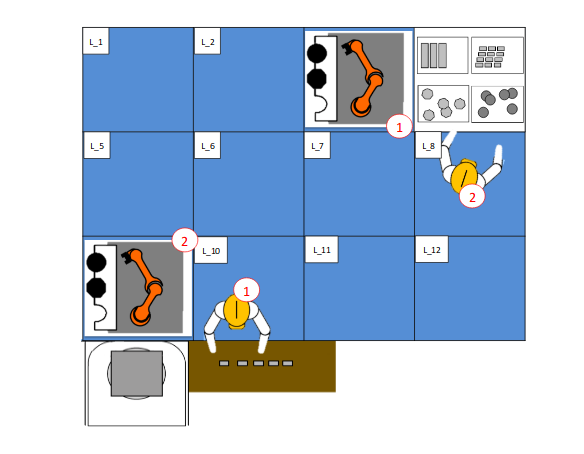
\includegraphics[width=\linewidth]{pictures/grid.png}
	\caption{The grid}
\end{figure}




\subsection{Document Structure}

This document is composed of three sections.
\begin{itemize}
	\item \textbf{Section1} Contains a general overview of the project
	\item \textbf{Section2} Contains description of the model in natural language
	\item \textbf{Section3} Contains the TRIO model
\end{itemize}
\clearpage

\section{Model description}
\subsection{Introduction}

\newpage
\subsection{Assumptions and Constraints}

\paragraph{Assumptions}
\newcommand{\DI}{\textbf{D1}: Position of the operator at next time instant is known}
\newcommand{\DII}{\textbf{D2}: There is no enforced time limit on the time that operator and robot stay still at their workstations}
\newcommand{\DIII}{\textbf{D3}: There is no enforced time limit on the time that operator and robot take to move between their workstations}
\newcommand{\DIV}{\textbf{D4}: }
\newcommand{\DV}{\textbf{D5}: }
\newcommand{\DVI}{\textbf{D6}: }
\newcommand{\DVII}{\textbf{D7}: }
\newcommand{\DVIII}{\textbf{D8}: }
\newcommand{\DIX}{\textbf{D9}: }
\newcommand{\DX}{\textbf{D10}: }
\newcommand{\DXI}{\textbf{D11}: }

The following assumptions have been taken into account while designing the model:
\newline\begin{itemize}
	\item  \DI
	\item  \DII
	\item  \DIII
%	\item  \DIV
%	\item  \DV
%	\item  \DVI
\end{itemize}

The domain assumption D1 means that the sensors present on the grid are not only able to detect if the operator is moving, but also \textit{where} it is going. This enables the robot controller to move quite efficiently in cells that are around the operator. This assumption could be removed but, in order to keep the safety property true, every instance in the controller of \textit{next(operatorIn(cell))}) would have to be replaced with a quantification over all the cells that the operator could potentially reach at the next time instant.
\newpage


\subsection{Robot Model}

The robot has been modeled as a 3-state FSM that governs the movement around the grid and is managed by a simple controller that is in charge of avoiding collisions. At each time instant the controller+FSM will consider the current state of the grid and force the updates of the robot state in the model.

Here follows a description of the actions taken for each state by the FSM:
\begin{itemize}
	\item \textbf{RobotToL9}: In this state the robot is going to L9
	\begin{itemize}
		\item \textbf{Next position is L9}: Transition to \textit{RobotWorking}
		\item \textbf{Next position is not L9}: Self loop
	\end{itemize}

	\item \textbf{RobotToL3}: In this state the robot is going to L3
	\begin{itemize}
		\item \textbf{Next position is L3}: Transition to \textit{RobotWorking}
		\item \textbf{Next position is not L3}: Self loop
	\end{itemize}

	\item \textbf{RobotWorking}: In this state the robot is working at a station
	\begin{itemize}
		\item \textbf{Working in L9}:
			\begin{itemize}
				\item \textbf{Next state is RobotToL3}: Move away
				\item \textbf{Next state is not RobotToL3}: Stay still
			\end{itemize}
		\item \textbf{Working in L3}:
			\begin{itemize}
				\item \textbf{Next state is RobotToL9}: Move away
				\item \textbf{Next state is not RobotToL9}: Stay still
			\end{itemize}
	\end{itemize}
\end{itemize}

It is a very simple representation and it is used mainly to keep track of what the robot was doing in the model.

The controller is made of four main axioms:
\begin{itemize}
	\item \textbf{Safety lock}: If the operator is in the same area as the robot, the controller prevents the robot from moving
	
	\item \textbf{Collision avoidance}: The controller prevents the robot from entering an area where the operator is at the same time instant
	
	\item \textbf{Detour avoidance(x2, one for L3 and one for L9)}: If the robot is one cell away from its destination the controller halts it until that cell is free, to avoid detours
\end{itemize}

As required by the specification document, the controller does not enforce a particular path to destination.

In addition to these, other axioms have been added in order to keep the grid model consistent with the specification:


\begin{itemize}
	\item \textbf{Forbidden place}: The robot cannot be in L4
	
	\item \textbf{Realistic movement}: The robot can only move by one cell at a time
	
	\item \textbf{Unique position}: The robot is in one and only one cell at each time instant
\end{itemize}

\subsection{Operator Model}
The operator has been modeled in the same way as the robot as far as the FSM is concerned. Since the operator is not an agent that is controllable by our system, it has no controller and can go wherever he or she wants: it will be the robot's duty to prevent accidents.

The FSM description is omitted as it is identical to the one given for the robot, just substituting L9 with L10 and L3 with L8 gives the operator's automaton.
As with the robot, axioms for model integrity have been added:

\begin{itemize}
	\item \textbf{Forbidden place}: The operator cannot be in L4
	
	\item \textbf{Realistic movement}: The operator can only move by one cell at a time
	
	\item \textbf{Unique position}: The operator is in one and only one cell at each time instant
\end{itemize}

\subsection{Simulation Model}
The simulation part of the model consists in four parts that are used to define the predicates used by operator and robot models and the safety property to be verified.

A complete specification is present in Section 3, but the main ones are:
\begin{itemize}
	\item \textbf{Init}: Initial conditions for the system
	\begin{itemize}
		\item Robot is in L3 in state RobotWorking
		\item Operator is in L10 in state OperatorWorking
	\end{itemize}
	
	\item \textbf{Collision Predicate}: A predicate that is true iff the robot and operator are in the same cell
	
	\item \textbf{Nice Simulation(Optional)}: Forces the simulation to do at least a loop for both the robot and operator. This is not guaranteed by just the model since the paths taken are left completely free from constraints and could never reach the destination cells within the set bound.
	
	
	\item \textbf{Collision Enforcing}: Enforces that sometime in the future there will be a collision with the robot moving into or out from the operator cell. This makes our model unsatisfiable, meaning that no such collision can happen.
	Since the specification states that collisions are to be avoided when the robot is moving, this model considers a "moving collision" to be the robot moving while the operator is in the same cell or moving to where the operator is (or will be at the next time instant).
\end{itemize}


\clearpage

\section{TRIO Model}
\subsection{Definitions}

In this specification some predicates taken from the \textit{Zot} syntax have been used. They can be easily reduced to basic TRIO predicates as follows:
\begin {itemize}
\item \textbf{Next(F)} = Dist(F,1)
\item \textbf{Yesterday(F)} = Dist(F,-1)

\end {itemize}

\subsection{Model}
This section contains the TRIO specification ....


%\lstinputlisting[language=Lisp]{../project.lisp}

\subsection{Verification}
AAA.....
\vspace{10mm}

Executing...
\clearpage

	
\end{document}
